\documentclass[]{article}
\usepackage{listings}
\usepackage{xcolor}
\usepackage{amssymb}
\usepackage{hyperref}
\usepackage{tikz}

%opening
\title{CSC373 Week 5 Tutorial}
\author{}

\begin{document}

\maketitle

\section{\href{http://www.geeksforgeeks.org/dynamic-programming-set-21-box-stacking-problem/}{Box-Stacking}}
Given a set of 3D boxes, how can we stack them in the highest way given the following rules?
\begin{itemize}
	\item A box, $A$, can only be stacked on another box, $B$,  if the base of $A$ is smaller than the base of $B$ (both depth and width)
	\item There are 3 different ways to rotate each box: \[(h,min(d,w),max(d,w))\] 
	\[(d,min(h,w),max(h,w))\]
	\[(w,min(d,h),max(d,h))\] 
	and we have an infinite supply of each rotation of each box.
	% The rest are symmetric and can be ignored as long as we keep some convension. another way is $(h,min(d,w),max(d,w)), (d,min(h,w),max(h,w)), (w,min(d,h),max(d,h))$.
\end{itemize}
%Use dynamic programming and create a 1D list of $3*n$ elements where $i$'th entry is the max height using the $i$'th box as the top box. Sort the boxes by base area then update/iterate $n$ times since the stack can have $n$ boxes at max. Only consider the boxes earlier in the list to stack on another, (since the base area is smaller). On each update, check if this new method produces a taller stack.

\section{\href{https://web.stanford.edu/class/archive/cs/cs161/cs161.1138/lectures/18/Small18.pdf}{Bellman-Ford}}
The Bellman-Ford algorithm can be used to find the shortest path tree from a single vertex. It is similar to Dijkstra's algorithm, in that regard, but it works on graphs with negative edges. Negative cycles, if found, cause the program to terminate since they create infinite loops.
%\textit{ Set the distance to each node to be infinity except the source, set to 0. Iterate over the following relaxation $n$ times (since the longest path has, at most, n edges). To relax a vertex, check if the distance to that vertex can be reduced by setting a new parent. If so, reduce the cost to that vertex and save the new parent.}

\begin{itemize}
	\item Trace how Dijkstra's algorithm runs on the graph below to see how it fails.
	\item Bonus: Trace how Bellman-Ford runs and try to find ways to improve it.
\end{itemize}

\begin{figure}
	\centering
	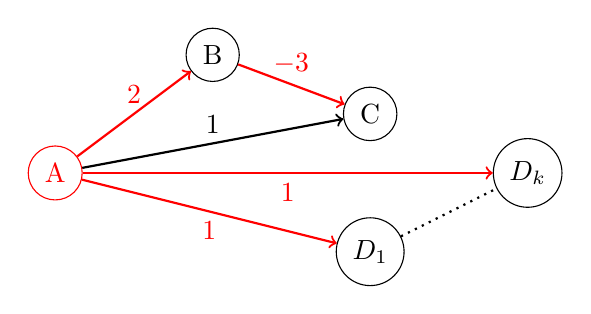
\begin{tikzpicture}
	\node[draw,circle,color=red] (A) at (0,-1.5) {A};
	\node[draw,circle] (B) at (2,0) {B};
	\node[draw,circle] (C) at (4,-.75) {C};
	\node[draw,circle] (Dk) at (6,-1.5) {$D_k$};
	\node[draw,circle] (D1) at (4,-2.5) {$D_1$};
	
	\draw [->, thick, color=red] (A) edge node[above] {$2$} (B);
	\draw [->, thick] (A) edge node[above] {$1$} (C);
	\draw [->, thick, color=red] (B) edge node[above] {$-3$} (C);
	
	\draw [->, thick, color=red] (A) edge node[below] {$1$} (D1);
	\draw [->, thick, color=red] (A) edge node[below] {$1$} (Dk);
	\draw [dotted, thick] (D1) edge node[below] {} (Dk);
	
	
	\end{tikzpicture}
	\caption{Graph with k-claw from $a$ to $D_i, 1 \leq i \leq k$. Shortest path tree from source $A$ is highlighted red}
\end{figure}
%\textit{If we get this far, the answer is \href{https://wcipeg.com/wiki/Shortest_Path_Faster_Algorithm}{Shortest Path Faster Algorithm (SPFA) aka Yen's improvement to Bellman-Ford}
%It is very similar, but it only updates vertices who have been updated in the current or last iteration. If they haven't been updated, then they cannot provide any new benefits.}
 
\end{document}
